%!TEX root = ../thesis.tex
%*******************************************************************************
%****************************** Fourth Chapter **********************************
%*******************************************************************************
\chapter{Evaluation and data analysis}

% **************************** Define Graphics Path **************************

\section{Introduction}

In an attempt to quantify the performance of the proposed system, a threefold evaluation was instantiated and conducted. This is presented in terms of the consistency of the LMC, followed by a comparative vector tolerance analysis and finally, the overall system accuracy. Thereafter a discussion is presented. The following evaluation and discussion are based on sample data that was collected through the scanning (enrolment and authentication) of forty unique candidates.

\section{Testing methodology}

%****************************************************************

In testing the system, it was decided that a simulation should be initiated in order to determine the reliability and efficiency of the system by eliminating the LMC. This was done due to the device's lack of customisability. As the system stored the transformed biometric data of the forty users within stego-image 2, the simulation would attempt to authenticate only the user data that was extracted during enrolment and authentication phases. 

In order to successfully simulate the authentication process, the following steps would need to be conducted: 

\begin{enumerate}[label=\roman*.]
    \item Both stego-images will be stored to read information from within the test program
    \item A list will be created correlating to the users PINs;
    \item A list will be created correlating to the transformed hand geometry extracted during the authentication scans;
    \item These lists will be iterated accordingly having each PIN in the list hashed and matched to the data corresponding to that PIN in stego-image 1;
    \item Once the PIN has successfully matched, the corresponding authentication transformation will be hashed and matched to the data within stego-image 2;
    \item Each of the aforementioned steps will be timed in order to gauge the efficiency of the matching algorithm.
    
\end{enumerate}

% Figure - Simulation authentication test
    
    \begin{figure}[htbp!] 
    \centering    
    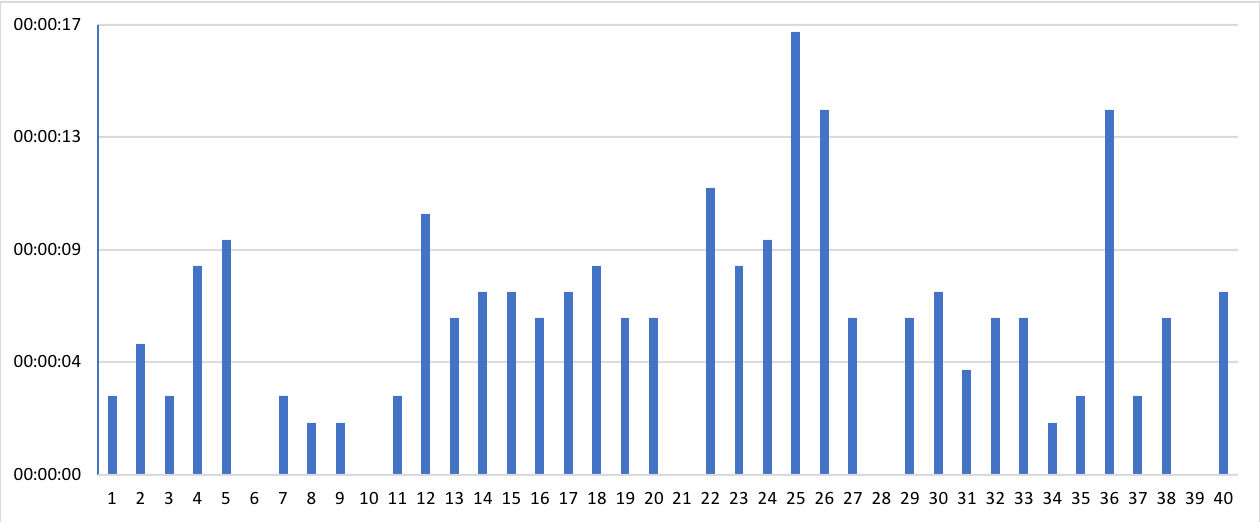
\includegraphics[width=1.0\textwidth]{Chapter4/Figs/AuthTest1.png}
    % \includesvg[width=0.8\textwidth]{Chapter4/Figs/AuthTest1.svg}
    \caption[Simulation for time taken to authenticate users]{Simulation for time taken to authenticate users}
    \label{fig:Simulation for time taken to authenticate users}
    \end{figure}
    
With the core functionality of the proposed system being to successfully transform and authenticate users, the efficiency is seen to be slightly lacking. As the above Figure \ref{fig:Simulation for time taken to authenticate users} shows, the algorithm used to find the authentication match within the threshold tolerance range of 5 affects the speed at which a user can be authenticated. A simple and effective solution to this drawback of obtaining a successful match may be to place an upper limit on the time that the algorithm is allowed to scan for a match for. This upper limit can be deduced from the average time taken to authenticate all forty users of 6,65s. 


\subsection{Leap Motion Controller performance evaluation}

To illustrate the efficiency and reliability of the LMC, the data that was collected from one randomly selected, five second hand geometry scan is presented in both Table~\ref{table: Randomly selected data from five second scan} and Figure~\ref{fig:Five Second hand scan graph} below. 
In order to present a visualisation with a high enough resolution to be able to see the variance in the scan readings, only the three fingers most similar in length are shown in Figure~\ref{fig:Five Second hand scan graph}(i.e., the index, middle, and ring fingers). 

% Table - Data from One, 5 second hand geometry scan
    
    \begin{table}[h!]
    \caption{Randomly selected data from five second scan}
    \centering
     \begin{tabular}{|p{0.18\textwidth} | p{0.18\textwidth}| p{0.18\textwidth}| p{0.18\textwidth}| p{0.18\textwidth}|} 
     \hline
    	\textbf{Thumb} & \textbf{Index} & \textbf{Middle} & \textbf{Ring} & \textbf{Pinky} \\ [1ex] 
     \hline\hline 
     0.197203783 & 0.424346553 &  0.464246258 & 0.438259197 & 0.35738522 \\[1ex]
     \hline 
     \end{tabular}
     \label{table: Randomly selected data from five second scan}
    \end{table}

% Figure - Five Second hand scan graph
    
    \begin{figure}[htbp!] 
    \centering    
    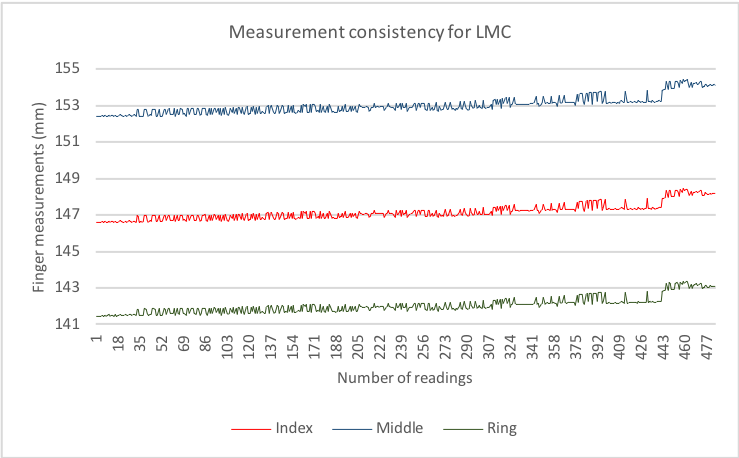
\includegraphics[width=1.0\textwidth]{Chapter4/Figs/Consistency.png}
    % \includesvg[width=0.8\textwidth]{Chapter4/Figs/Figure1.svg}
    \caption[Five Second hand scan graph]{Five Second hand scan graph}
    \label{fig:Five Second hand scan graph}
    \end{figure}
    
The significance of this data is prevalent when taking into consideration the distribution throughout the scan. It is of utmost importance to conistently extract concise data readings throughout the length of the scan. Thus, the standard deviation of the raw data correlating to the plotted data was calculated in an attempt to demonstrate the accuracy that the LMC provides (see Table~\ref{table: Randomly selected data from five second scan}).

It is interesting to note that the longer the scan has progressed, the more varied the readings become. This is attributed to the instability that is associated with an unsupported hand being held in mid-air for any given period of time.

\subsection{Comparitive vector tolerance}

Despite the above-mentioned LMC accuracy, the system shows slight deviation from one scan to the next. To provide an explicit limit regarding the deviation of the readings during a scan, it was decided to measure a tolerance range.

The manner within which this tolerance range was calculated involves comparing test data from user enrolment scan to that of the associated authentication scan. This data includes all of the users and their transformed vector combinations. With this data, the maximum tolerance range was extrapolated based on the variations produced by the system. As seen in Figure~\ref{fig:Comparative vector tolerance} below, it was concluded that the maximum tolerance range for this data set is 5mm.

% Figure - Comparative vector tolerance
    
    \begin{figure}[htbp!] 
    \centering    
    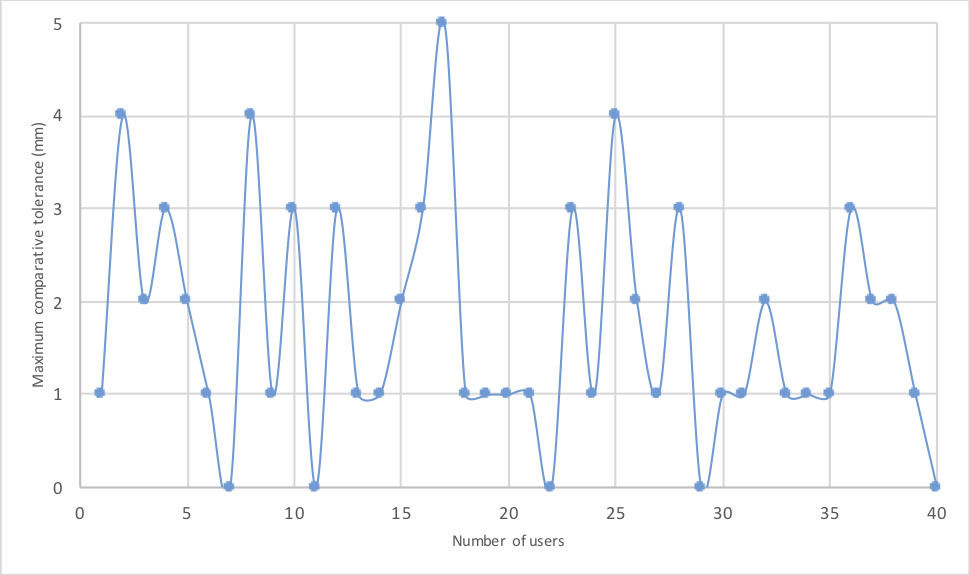
\includegraphics[width=1.0\textwidth]{Chapter4/Figs/Comparative.png}
    % \includesvg[width=1\textwidth]{Chapter4/SVG/Comparative-pdf.svg}
    \caption[Comparative vector tolerance]{Comparative vector tolerance}
    \label{fig:Comparative vector tolerance}
    \end{figure}

Upon further evaluation, with the tolerance range at a maximum of 5mm, the acceptance rates exponentially improved. This, however, increased the processing time to find a positive match within the tolerance range of the transformed vector. 

\section{Algorithm evaluation}

As with any authentication system, one needs to take into consideration human error or inconsistency during the scanning process. To better illustrate the thought process prior to the formulation of the Algorithm \ref{algorithm: Recursive algorithm to find possible vector combinations}, consider the following example:

\begin{enumerate}[label=\roman*.]
    \item User A enrols with the transformed hand geometry vector of {50, 60, 70, 80, 90};
    \item When the user A attempts to authenticate thereafter, his/her hand is not scanned identically due to various factors and the transformed hand geometry vector produced this time is {52, 59, 74, 81, 90}
    \item Due to the SHA-256 hashing applied to the transformed geometry prior to storage, the match to the value stored within stego-image 2 fails, even though user A has provided the correct PIN.
    \item In order to provide greater match accuracy, an algorithm was formulated in order to compensate for fault tolerance during scans.
    \item As seen in Figure \ref{fig:Comparative vector tolerance}, the fault tolerance was variable for a range of 5 for each vector value.
\end{enumerate}

With a fault tolerance of 5mm, the probability of finding an exact match of the stored biometric increases exponentially. Algorithm~\ref{algorithm: Recursive algorithm to find possible vector combinations} attempts to find a match as efficiently as possible while reducing the amount of false positive matches produced by the system.

Once the scanned vector is passed into this algorithm, the calculations proceed as follows:

\begin{enumerate}[label=\roman*.]
    \item The original transformed vector is copied and the 1st value is decremented by 1;
    \item This alteration creates a new vector;
    \item This vector is then hashed and compared to what is stored in stego-image 2.
    \item The process repeats itself for each value until the last value in the original vector is decremented by 1;
    \item The 1st value is then incremented by 1, hashed and compared to what is stored in stego-image 2;
    \item The process then repeats itself and increases the increment to 2, 3, 4 and 5 respectively;
    \item If a match is found during this process, the algorithm is halted. If no match is found, the algorithm continues to recursively search for a match until the possible vector combinations are exhausted.
\end{enumerate}

The above-mentioned process is illustrated below in Algorithm~\ref{algorithm: Recursive algorithm to find possible vector combinations}.
% Algorithm - check vector hash combinations

\begin{algorithm}
     \SetKwInOut{Input}{Input}
     \SetKwInOut{Output}{Output}
     
     \underline{function VectorCombinationsCheck} ( $transformedVector$, $count$)\;
     \Input{$transformedVector$}
     \Output{$result$}
     
      \tcp{transformedVector, low and high are \textbf{vectors}}
      $low$;
      $high$;
     
     $increment$ = 0;
     
     \If{$count$ = $transformedVector$.Length}{
        \textbf{return}\;
     }
     
     \For{($value$ in $transformedVector$)}{
        $increment$++\;
        
        \textbf{Array}.Copy($transformedVector$, $low$)\;
        $low$[count] = $transformedVector$[count] - $increment$\;
        \textbf{checkLowMatch} = GenerateHash($low$)\;
        \textbf{Array}.Copy($transformedVector$, $high$)\;
        $high$[count] = $transformedVector$[count] + $increment$\;
        \textbf{checkHighMatch} = GenerateHash($high$);
        \tcp{Recurse}
        \textbf{VectorCombinationsCheck}($low$, count + 1)\;
        \textbf{VectorCombinationsCheck}($high$, count + 1)\;
        
     }
     
     return $result$ = \textbf{VectorCombinationsCheck($transformedVector$)}
     
     \label{algorithm: Recursive algorithm to find possible vector combinations}
     \caption{Recursive algorithm to find possible vector combinations}
\end{algorithm}

This approach attempts to decrease the false-positive match rates. 

%****************************************************************

\subsection{Overall system evaluation}

As deduced from Figure~\ref{fig:System tolerance versus acceptance rates}, a 0mm tolerance rate resulted in only a 12.5\% true acceptance rate. If this tolerance is then increased, the true acceptance rate also increases (e.g. 97.5\% with a 4mm tolerance) until a 100\% true acceptance rate is obtained at 5mm tolerance. 
When considering implementing this particular system approach, one needs to determine what risk factor is suitable within the authentication scenario. If the users that need to be authenticated are to be granted access to sensitive data/areas, then the tolerance range should be adjusted accordingly. The acceptance rate is drastically affected when using the maximum tolerance range. With such a high tolerance range, the false acceptance rate is also dramatically increased, but because of the two-factor authentication provided with the allocated PIN, the users are authenticated correctly and no inter-user error is observed where one user is authenticated as another.

% Figure - System tolerance vs acceptance rates
    
    \begin{figure}[htbp!] 
    \centering    
    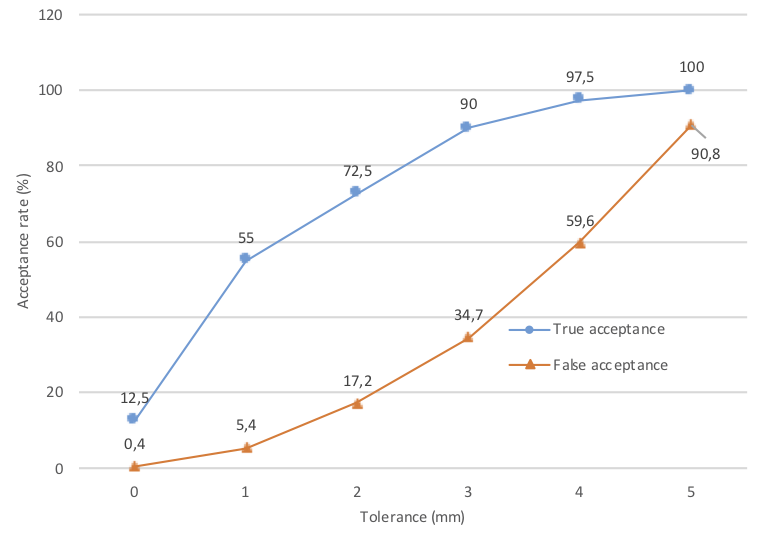
\includegraphics[width=1.0\textwidth]{Chapter4/Figs/Tolerance.png}
    % \includesvg[width=1\textwidth]{Chapter4/SVG/Tolerance-pdf.svg}
    \caption[System tolerance versus acceptance rates]{System tolerance versus acceptance rates}
    \label{fig:System tolerance versus acceptance rates}
    \end{figure}


\section{Discussion}

The proposed technique has revealed several promising advantages by using a combination of the techniques specified in Chapter 2. The LMC was found to be a stable and efficient hand geometry scanner. Also, the steganography techniques used in this paper were relatively easy to implement for use in this particular instance. By using PINs (to implement two-factor authentication) the security is enhanced and aids in achieving cancelability for storing biometrics. The proposed framework ensured that the system provided results that were reliable and efficiently obtained.

Bearing in mind the above-mentioned advantages, some disadvantages are present when using this approach. The algorithm to find positive matches slowed down the system. It may be of value to consider the possibility of removing the algorithm in future and alternatively producing a false match, followed by a re-scan. This system was only exposed to limited testing and the authentication accuracy and robustness will need to be measured using a formal evaluation. In order to fully explore the system’s functionality, extensive tests should be conducted upon this framework on a larger scale. This will form part of the ongoing research.


\section{Chapter summary}

The aim of this chapter was to evaluate the overall system design, performance, accuracy and efficiency. This was done by analysing data extracted during the testing process. Once analysis on that data was complete, the system performance, accuracy and efficiency was measured using simulation tests by removing certain system components. The algorithmic complexity was analysed for optimisation possibilities.

In Chapter 5, the objectives of the study will be revisited and discussed. Any problems experienced throughout the study will also be addressed and opportunities that may have come to fruition throughout the research will be discussed for future studies.